%%%%%%%%%%%%%%%%%%%%%%%%%%%%%%%%%%%%%%%%%%%%%%%%%%%%%%%%%%%%
%\documentclass[xcolor=x11names,compress]{beamer}
\documentclass[handout]{beamer}
\definecolor{CoolBlack}{rgb}{0.0, 0.18, 0.39}
\definecolor{byellow}{rgb}{0.55037, 0.38821, 0.06142}
%% General document %%%%%%%%%%%%%%%%%%%%%%%%%%%%%%%%%%
\usepackage{graphicx}
\usepackage{tikz}
\usepackage{Tabbing, tabu}
\usetikzlibrary{decorations.fractals}
%%%%%%%%%%%%%%%%%%%%%%%%%%%%%%%%%%%%%%%%%%%%%%%%%%%%%%

%% Beamer Layout %%%%%%%%%%%%%%%%%%%%%%%%%%%%%%%%%%
\useoutertheme[subsection=false,shadow]{miniframes}
\useinnertheme{default}
\usefonttheme{serif}
\usepackage{palatino}
\usepackage{tabu}

% addition of color
\usepackage{xcolor}
\definecolor{dgreen}{rgb}{0.,0.6,0.}
\definecolor{RawSienna}{cmyk}{0,0.72,1,0.45}

\setbeamerfont{title like}{shape=\scshape}
\setbeamerfont{frametitle}{shape=\scshape}

\setbeamercolor*{lower separation line head}{bg=CoolBlack} 
\setbeamercolor*{normal text}{fg=black,bg=white} 
\setbeamercolor*{alerted text}{fg=dgreen} 
\setbeamercolor*{example text}{fg=black} 
\setbeamercolor*{structure}{fg=black} 
 
\setbeamercolor*{palette tertiary}{fg=black,bg=black!10} 
\setbeamercolor*{palette quaternary}{fg=black,bg=black!10} 

% Links
\usepackage{hyperref}
\definecolor{links}{HTML}{003262}
\hypersetup{colorlinks,linkcolor=,urlcolor=links}

% columns
\renewcommand{\(}{\begin{columns}}
\renewcommand{\)}{\end{columns}}
\newcommand{\<}[1]{\begin{column}{#1}}
\renewcommand{\>}{\end{column}}

% adding slide numbers
\addtobeamertemplate{navigation symbols}{}{%
    \usebeamerfont{footline}%
    \usebeamercolor[fg]{footline}%
    \hspace{1em}%
    \insertframenumber/\inserttotalframenumber
}

% equation stuff
\newcommand{\Macro}{\ensuremath{\Sigma}}
\newcommand{\Sn}{\ensuremath{S_N} }
\newcommand{\vOmega}{\ensuremath{\hat{\Omega}}}
\usepackage{mathrsfs}
\usepackage[mathcal]{euscript}
\usepackage{amssymb}
\usepackage{amsthm}
\usepackage{epsfig}
\usepackage{amsmath}

\newcommand{\ve}[1]{\ensuremath{\mathbf{#1}}}
\newcommand{\micro}{\ensuremath{\sigma}}
\newcommand{\detR}{\ensuremath{\Sigma}}

\newcommand\RBox[1]{%
  \tikz\node[draw,rounded corners,align=center,] {#1};}%

\setbeamerfont{author in head/foot}{size={\fontsize{3pt}{4pt}\selectfont}}
%\author[Subham \& Mithun \& Karthikeyan \& Shantikumar]
%{%
%   \texorpdfstring{
%        \begin{columns}
%            \column{.25\linewidth}
%            \centering
%            \includegraphics[height=3cm]{../bk-eps-converted-to}
%            \column{.25\linewidth}
%            \centering
%            \RBox{R.\ N.\ Slaybaugh\\
%            Univ.\ of Cal.\ Berkeley}\\[1ex]
%            \RBox{T.\ M.\ Evans, and\\
%            S.\ W.\ Mosher\\
%            Oak Ridge National Lab}
%        \end{columns}
%   }
%   {Subham Soni S., Karthikeyanm, Shantikumar L.,  Mithun C.K.}
%}
\title{Improved Hybrid Modeling}
\subtitle{of Used Fuel Storage Facilities}
\author{\includegraphics[height=2cm]
{../bk-eps-converted-to}\\R.\ N.\ Slaybaugh, Univ.\ of Cal.\ Berkeley\\[1ex]
T.\ M.\ Evans and S.\ W.\ Mosher, Oak Ridge National Lab}
\date{17 March 2016 \\ DOE MPACT Meeting}

%%%%%%%%%%%%%%%%%%%%%%%%%%%%%%%%%%%%%%%%%%%%%%%%%%

\begin{document}

%%%%%%%%%%%%%%%%%%%%%%%%%%%%%%%%%%%%%%%%%%%%%%%%%%%%%%
%%%%%%%%%%%%%%%%%%%%%%%%%%%%%%%%%%%%%%%%%%%%%%%%%%%%%%
\begin{frame}
\titlepage
\end{frame}

% --------------------------------------------------------------
\begin{frame}[fragile]{Outline}
  \frametitle{Outline}

\begin{columns}
  \begin{column}{0.5\textwidth}
    \begin{itemize}
    \item Motivation
    \vspace*{.75em}
    \item Hybrid Methods and Strong Anisotropies
    \vspace*{.75em}
	\item New Method
    \vspace*{.75em}
	\item Initial Results and Plans
  \end{itemize}
  \end{column}
  \begin{column}{0.5\textwidth}
  	\begin{figure}
  	\begin{center}
  		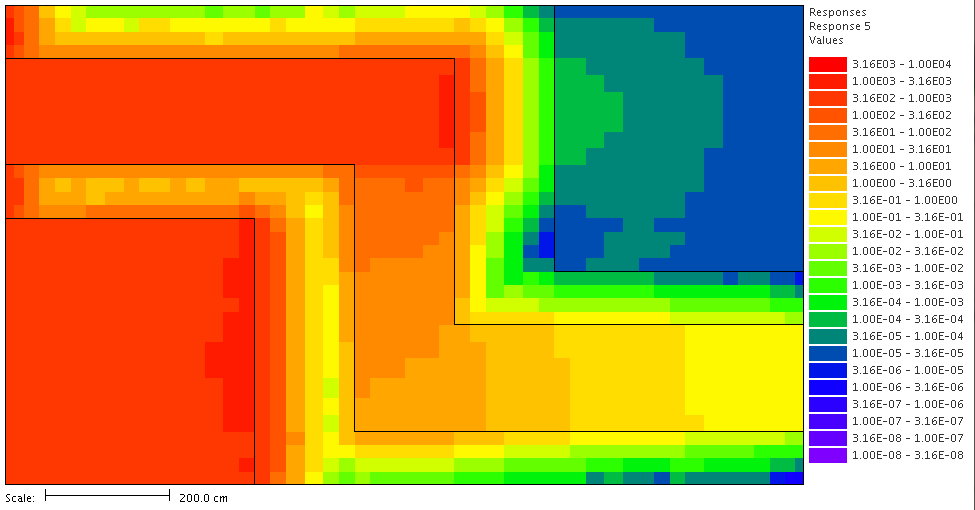
\includegraphics[height=1.1in,clip]{../figs/labyrinth-dr}
		\caption{Radiation dose in challenging geometry}
		%For particles near the turns in the labyrinth, the importance of the particles to the exit of the labyrinth vary greatly if they are coming out of a wall pointed toward the exit versus heading into a wall and away from the exit. This distinction is not captured by current hybrid methods. 
	\end{center}
  	\end{figure}
  \end{column}
\end{columns}

\end{frame}


% --------------------------------------------------------------
% --------------------------------------------------------------
\section{\scshape Motivation}
\begin{frame}[fragile]
  \frametitle{Project motivation}

\begin{columns}
  \begin{column}{0.55\textwidth}
	\begin{itemize}
	\item Need to accurately model radiation for safeguarding and monitoring
	\item \alert{Challenging}: dense shields; streaming paths
	\item Current methods are insufficient
	\item \alert{Goal}: accurate solutions in reasonable time
	\item New methods can easily be added to existing codes
	\end{itemize}
  \end{column}
  \begin{column}{0.45\textwidth}
  	\begin{figure}
  	\begin{center}
  		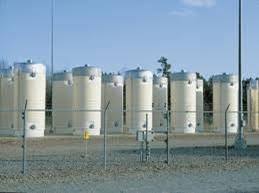
\includegraphics[height=1.25in,clip]{../figs/isfsi}
		\caption{Used fuel storage pad}
	\end{center}
  	\end{figure}
  \end{column}
\end{columns}

\end{frame}

% --------------------------------------------------------------
% --------------------------------------------------------------
\begin{frame}[fragile]
  \frametitle{Solving the TE}
%
\begin{columns}
  \begin{column}{0.5\textwidth}
  \begin{center}
  \underline{Monte Carlo}
  \end{center}
	\begin{itemize}
	\item Solution has statistical error
	\item \textit{Continuous} phase space%: ``gold standard answers"
	\item Can be slow
	\item Optically thick = \textit{slow}
	\end{itemize}
  \end{column}
  \begin{column}{0.5\textwidth}
  \begin{center}
  \underline{Deterministic}
  \end{center}
	\begin{itemize}
	\item Solution equally valid everywhere
	\item \textit{Discretized} phase space%: drives solution quality
	\item Can be fast
	\item Streaming = \textit{ray effects}
	\end{itemize}
  \end{column}
\end{columns}
%
\begin{align}
\vOmega \cdot \nabla \psi(\vec{r}, E, \vOmega) &+
\Sigma_t \psi(\vec{r}, E, \vOmega) = S(\vec{r}, E, \vOmega) \:+\nonumber\\
%
& \int_{4\pi} d\vOmega' \int_0^{\infty} dE'\: \Sigma_s(E', \vOmega' \rightarrow E, \vOmega) \psi(\vec{r}, E', \vOmega') \nonumber
\end{align}

\end{frame}

% --------------------------------------------------------------
\begin{frame}[fragile]
  \frametitle{Speeding up MC}
  \begin{itemize}
	\item Variance reduction (VR) used to improve Monte Carlo:\\
	reduce relative error \textit{and} time by augmenting game
	\item Particles are assigned weights that map to impact
	\item VR can be used to
	  \begin{itemize}
	  \item set weights at birth
	  \item update weights throughout problem
      \end{itemize}
      \pause
  \item Improvement measured as    
  \end{itemize}
\[
\text{FOM} = \frac{1}{\text{R}^2\text{t}} \quad \text{R = relative error;  t = time} 
\]
\pause
\textbf{Hybrid Methods:} we use deterministic results to make Monte Carlo VR parameters

\end{frame}


% --------------------------------------------------------------
% --------------------------------------------------------------
\section{\scshape Strong Anisotropies}
\begin{frame}[fragile]
  \frametitle{Anisotropy: a computational challenge}

	\begin{columns}
  	\begin{column}{0.5\textwidth}
	\begin{itemize}
	\item Many important nuclear applications have strong anisotropies
	 \begin{itemize}
	 \item \textbf{Used fuel casks}
	 \item Reprocessing facilities
	 \item Reactor facilities
	 \item Active interrogation 
	 \end{itemize}
	\pause
	\item New ideas are needed for these problems
	\begin{itemize}
	\item Current hybrid methods are insufficient
	\item Including angle explicitly is too costly	
	\end{itemize}
	\end{itemize}
  	\end{column}
 	%
 	\begin{column}{0.5\textwidth}
 	 \begin{center}
 	 \begin{figure}
 	 \includegraphics[height=2in,clip]{../figs/pwr}  
 	 \caption{PWR relative error \cite{Pantelias2013}}
 	 \end{figure}
 	 \end{center}

  	\end{column}
	\end{columns}

\end{frame}


% --------------------------------------------------------------
\begin{frame}[fragile]
  \frametitle{Adjoint as an importance map}
Use \textit{adjoint}: the importance of a source particle to the solution

\begin{itemize}
\item Forward ($\phi$ or $\psi$): neutrons flow from the source to the detector
\item Adjoint($\phi^{\dagger}$ or $\psi^{\dagger}$): particles represent how each part of phase space contributes to the ``source"
\item The current state of the art is FW/CADIS \cite{Wagner2007}
\end{itemize}
\begin{align*}
  imp(\ve{r}, E) &= \frac{\phi^{\dagger}(\ve{r}, E)}{\langle q(\ve{r}, E), \phi^{\dagger}(\ve{r}, E) \rangle} = \frac{\phi^{\dagger}(\ve{r}, E)}{R} \\
  %
  \hat{q}(\ve{r}, E) &= \frac{\phi^{\dagger}(\ve{r}, E) q(\ve{r}, E)}{R} \\
  %
  w_0(\ve{r}, E) &= \frac{q(\ve{r}, E)}{\hat{q}(\ve{r}, E)} = \frac{R}{\phi^{\dagger}(\ve{r}, E)} 
\end{align*}

\end{frame}


% --------------------------------------------------------------
\begin{frame}[fragile]
  \frametitle{Current hybrid methods are insufficient}

\[\text{Note:}\qquad\phi^{\dagger}(\ve{r},E) = \int \psi^{\dagger}(\vOmega, 
		\ve{r},E) d\vOmega\]

	\begin{itemize}
	\item MC VR parameters created from adjoint deterministic scalar flux that is a function of \textit{space and energy only} \vspace*{1 em}
	\pause
	\item Angular dependence of the importance function is not retained, otherwise the map would be 
	\begin{itemize}
	  \item very large (tens or hundreds of GB) and
	  \item more costly and complex to use in the MC simulation 
	\end{itemize}
	\pause
	\item Drawback: within a given space/energy cell, map provides average importance of a particle moving in \textit{any direction} through the cell--excluding information about how particles move \alert{toward the objective}
	\end{itemize}

\end{frame}

% --------------------------------------------------------------
\begin{frame}[fragile]
  \frametitle{Current hybrid methods are insufficient}

	\begin{columns}
  	\begin{column}{0.5\textwidth}
 	 \begin{center}
 	 \begin{figure}
 	 \includegraphics[height=2in,clip]{../figs/boat-interrogation}  
 	 \caption{Spherical boat model with source on left and fissionable material at center}
 	 \end{figure}
 	 \end{center}
  	\end{column}
 	%
 	\begin{column}{0.5\textwidth}
 	 \begin{center}
 	 \begin{figure}
 	 \includegraphics[height=2in,clip]{../figs/boat-map}  
 	 \caption{Target weight window values for 14.1 MeV neutrons}
 	 \end{figure}
 	 \end{center}
  	\end{column}
	\end{columns}

\end{frame}


% --------------------------------------------------------------
\section{\scshape New Method}
\begin{frame}[fragile]
  \frametitle{Integration weighting}

    Different integration plan captures angles in scalar flux creation	
	\begin{align*}
		\phi^{\dagger}(\ve{r},E) &= \int \psi^{\dagger}(\vOmega, 
		\ve{r},E) d\vOmega \qquad  \qquad \qquad \text{original}\\
		 %
		\phi^{\dagger}(\ve{r},E) &= \frac{\int \psi(\vOmega, \ve{r},E)
		 \psi^{\dagger}(\vOmega, \ve{r},E) d\vOmega}{\int \psi(\vOmega, 
		 \ve{r},E)  d\vOmega} \qquad \text{\alert{new}}
	\end{align*}
%Note that these two calculations can be completed concurrently. Then, the adjoint scalar fluxes will be computed by angularly integrating the product of the forward and adjoint angular fluxes to account for the directions in which the particles will actually be traveling at any given location/energy:
%will provide importance values that more accurately reflect the average importance of particles that will be transported in the final Monte Carlo calculation, yielding faster Monte Carlo run times.
    \pause
    Major challenges and areas of investigation:
	\begin{enumerate}
	\item Data storage and handling (many GBs)
	\item More, less, or differently sensitive to 
	  \begin{itemize}
	  \item quality of the discrete ordinates calculation?
	  \item ray effects?
	  \end{itemize}
	\end{enumerate}

\end{frame}


% --------------------------------------------------------------
\begin{frame}[fragile]
  \frametitle{Method implementation}

  	\begin{itemize}
    \item The space- and energy-dependent importance map is normalized and 
     source biasing parameters are generated in the \alert{same ways} as
     the current implementation of FW/CADIS \vspace*{1 em}
	\item Immediately useful; widely applicable \vspace*{1 em}
	\item We are studying and characterizing the impact\vspace*{1 em}
	\item Will be available in ADVANTG \cite{Pantelias2013}
	\end{itemize}
	
\end{frame}


% --------------------------------------------------------------
% --------------------------------------------------------------
\section{\scshape Results and Plans}
\begin{frame}[fragile]
  \frametitle{Status and Plans}

    \begin{enumerate}
    \item Implementation: nearly complete
      \begin{itemize}
      %\item Large data handling is \alert{broader outcome}
      \item Implementation of weighted flux algorithm% in Denovo \cite{Evans2010}
       \alert{complete}
      \item Integration of method into ADVANTG \alert{underway}
      \item ADVANTG allows for ease of use; broader user base
      %\item Denovo integration enhances use on other hybrid platforms
      \end{itemize} 
      \vspace*{0.5em}
      \pause
    \item Testing: initiating
      \begin{itemize}
      \item Compare to existing methods
      \item Study performance around angular discretization
      \item Undergrad running existing methods; grad student developing tests
      \end{itemize}
      \vspace*{0.5em}
      \pause
    \item Impact characterization: planned
      \begin{itemize}
      \item Investigate performance for one used fuel canister
      \item Investigate performance for array of used fuel canisters
      \item \alert{Goal}: improved material control and accountability
      \end{itemize}
    \end{enumerate}

	
\end{frame}

% --------------------------------------------------------------
% --------------------------------------------------------------
%\section{\scshape Initial Results}
\begin{frame}[fragile]

  \frametitle{Results 1: maze problem}
  10 MeV isotropic point source
  \begin{columns}
   \begin{column}{0.45\textwidth}
   \begin{itemize}
\item Concrete maze
\item Air duct
\end{itemize}
   \end{column}
  %
  \begin{column}{0.5\textwidth}
   \begin{itemize}
\item NaI detector; 26 groups
\item Reflecting BCs
\end{itemize}
   \end{column}
\end{columns}
   \begin{figure}
   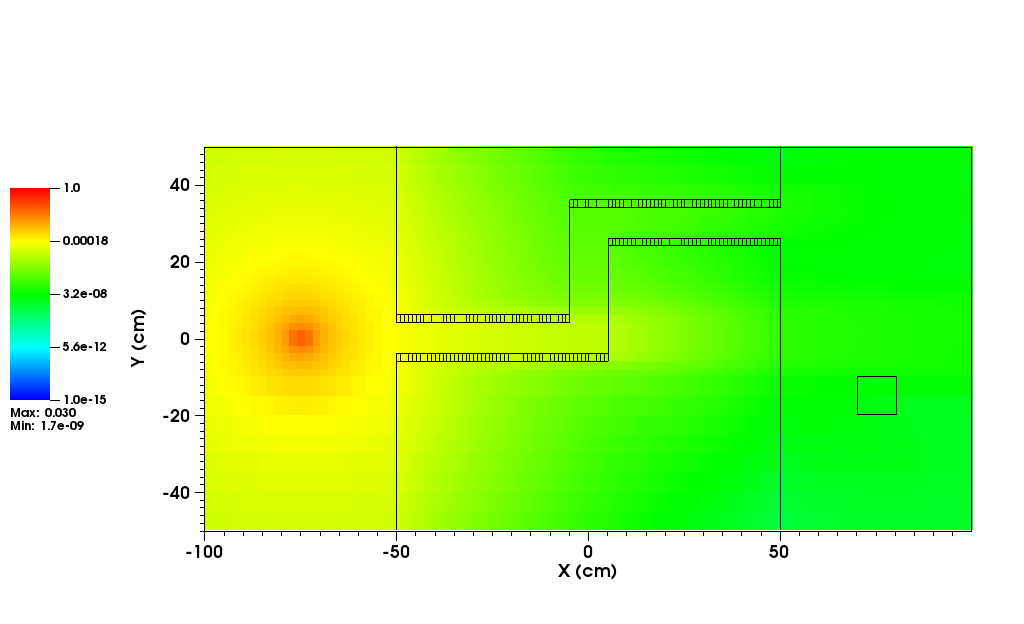
\includegraphics[height=2in,clip]{maze2_forward_group00_adjusted.png}
   %\caption{Simple two-turn labyrinth}
   \end{figure}


	
\end{frame}

%% --------------------------------------------------------------
%
\begin{frame}[fragile]
  \frametitle{Quantifying Anisotropy}
  
    \begin{columns}
    \begin{column}{0.5\textwidth}
  	\begin{figure}
  	\begin{center}
  		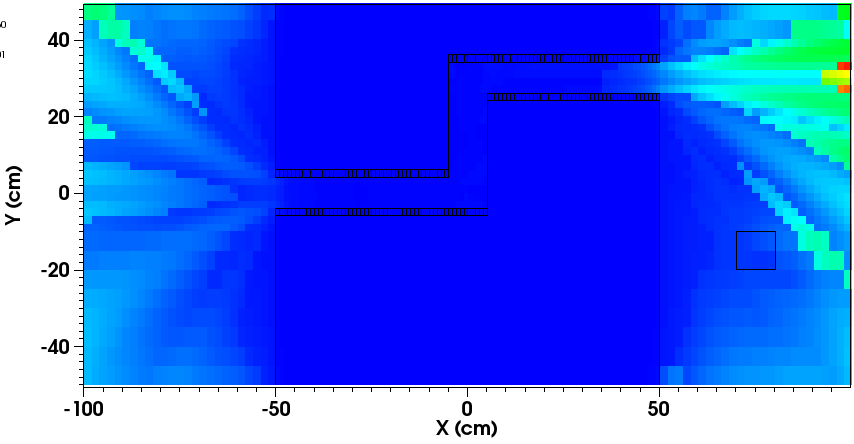
\includegraphics[height=1.1in,clip]{maze2_anisotropy_forward_group26_cropped.png}
		%\caption{Forward flux anisotropy}
	\end{center}
  	\end{figure}
  	  \begin{figure}
  	\begin{center}
  		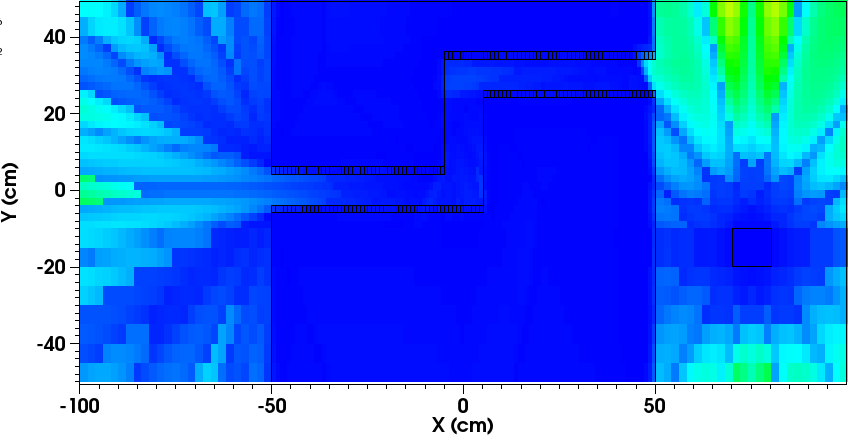
\includegraphics[height=1.1in,clip]{maze2_anisotropy_adjoint_group26_cropped.png}
		%\caption{Adjoint flux anisotropy}
	\end{center}
  	\end{figure}
    \end{column}
  \pause
    \begin{column}{0.5\textwidth}
    Combining forward and adjoint fluxes, we see:
    \begin{itemize}
        \item Some elimination of ray effects
        \item Anisotropy captured 
    \end{itemize}
  	\begin{figure}
  	\begin{center}
  		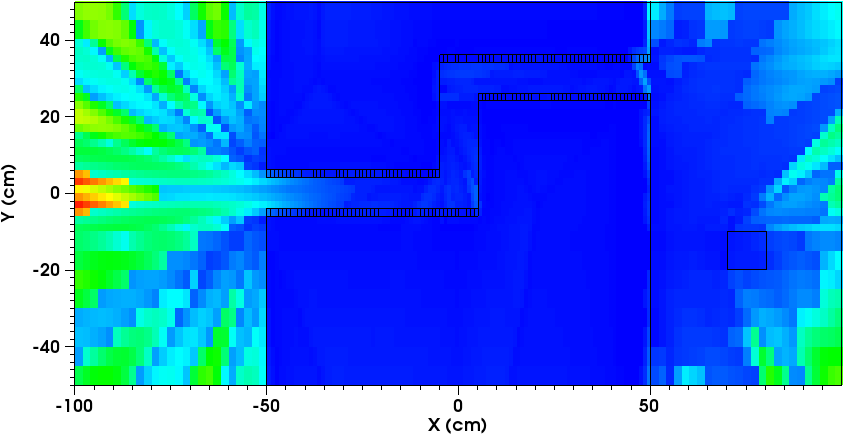
\includegraphics[height=1.1in,clip]{maze2_anisotropy_contributon_group26_cropped.png}
		%\caption{Contributon flux anisotropy }
	\end{center}
  	\end{figure}
  	\end{column}  
  \end{columns}
\end{frame}

%% --------------------------------------------------------------

\begin{frame}[fragile]
  \frametitle{Generating adjusted fluxes}
  %However, the method is not dominated by \textbf{just} the anisotropy....
  \begin{columns}
    \begin{column}{0.5\textwidth}
  	\begin{figure}
  	\begin{center}
  		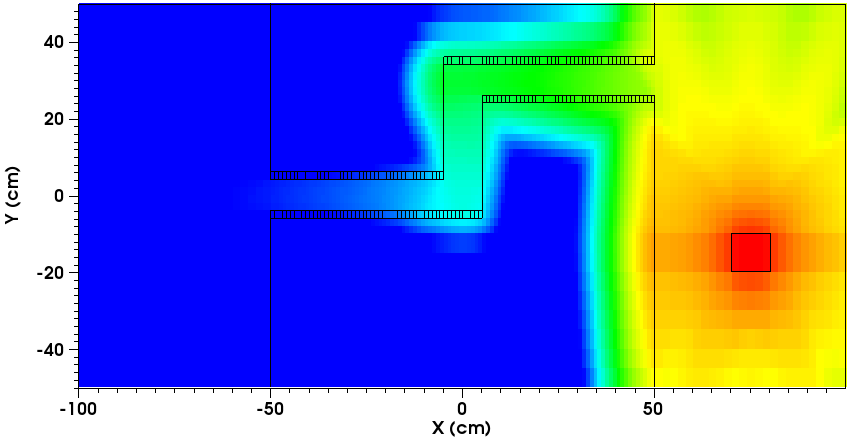
\includegraphics[height=1.1in,clip]{maze2_adjoint_group26_adjusted_cropped.png}
		%\caption{Regions with high importance}
	\end{center}
  	\end{figure}
  	  \begin{figure}
  	\begin{center}
  		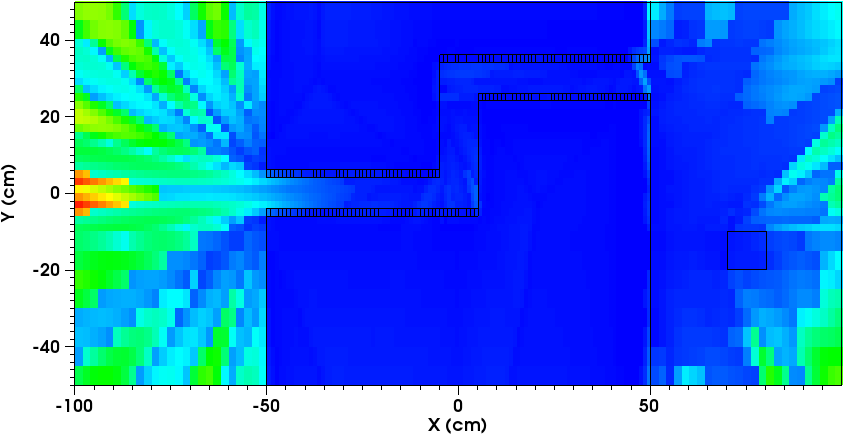
\includegraphics[height=1.1in,clip]{maze2_anisotropy_contributon_group26_cropped.png}
		%\caption{... coupled with strong anisotropies}
		% point out that while the FOM is better for analog, it has high RE in regions, so overall it performs poorer
	\end{center}
  	\end{figure}
    \end{column}
  \pause
    \begin{column}{0.5\textwidth}
   Regions with high importance coupled with strong anisotropy result in adjusted flux incorporating both
  	\begin{figure}
  	\begin{center}
  		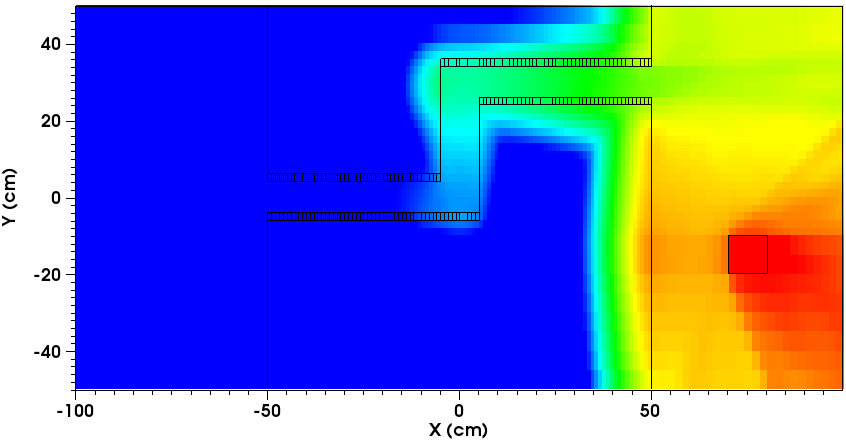
\includegraphics[height=1.1in,clip]{maze2_myflux_group26_adjusted_cropped.png}
		%\caption{Result in adjusted flux incorporating both }
	\end{center}
  	\end{figure}
  	\end{column}  
  \end{columns}
  %\alert{The new method incorporates both importance AND anisotropy into weighting parameters}
\end{frame}

%% --------------------------------------------------------------

\begin{frame}[fragile]
  \frametitle{Adjusted Fluxes}


	Comparing the original adjoint to CADIS-$\Omega$....
	\vspace*{1 em}
	\begin{columns}
  	\begin{column}{0.5\textwidth}
  	\begin{figure}
  	\begin{center}
  		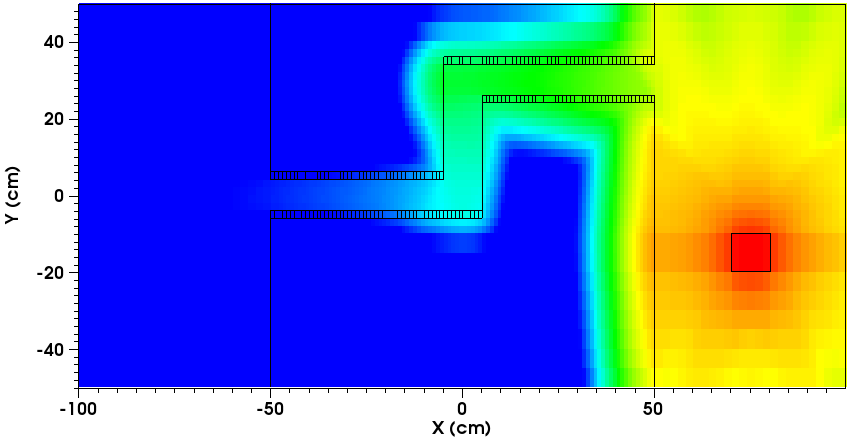
\includegraphics[height=1in,clip]{maze2_adjoint_group26_adjusted_cropped.png}
		%\caption{Adjoint flux used by CADIS}
	\end{center}
  	\end{figure}
  	\end{column}
 	%
 	\begin{column}{0.5\textwidth}
 	\begin{figure}
  	\begin{center}
  		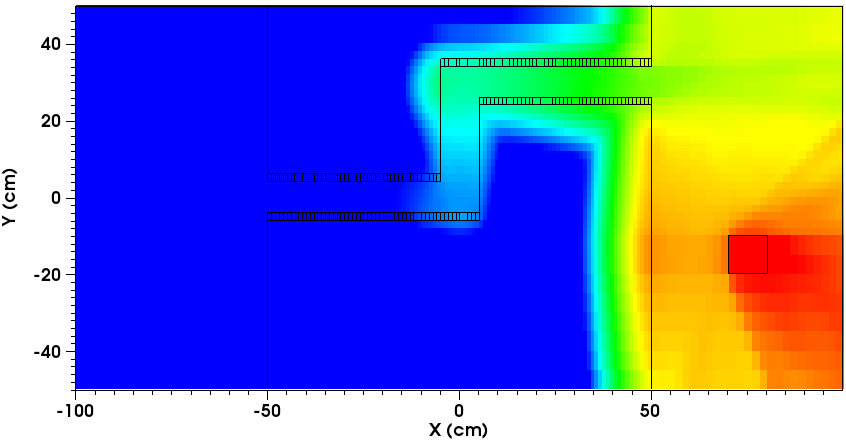
\includegraphics[height=1in,clip]{maze2_myflux_group26_adjusted_cropped.png}
  		%\caption{Adjoint flux used by CADIS-$\Omega$}
  	\end{center}
  	\end{figure}
  	\end{column}
	\end{columns}
	\vspace*{1 em}
	.... shows that the method does incorporate problem physics differently
  
	
\end{frame}

%% --------------------------------------------------------------
%
\begin{frame}[fragile]
  \frametitle{Response in detector}
  
\begin{columns}
  \begin{column}{0.45\textwidth}
  Adjusted CADIS has:
  \begin{itemize}
    \item Relatively uniform uncertainty distribution
    \item Raster runtimes than CADIS
    \item Better overall results than analog
  \end{itemize}
  \begin{tabular}{|l|c c|}
  \hline
      Run Type & FOM$_{MC}$ & FOM$_{adj}$ \\  
      \hline
      Analog & 493 & 493 \\
      CADIS  & 8   &   7 \\
      CADIS-$\Omega$ & 466 & 354 \\
      \hline
  \end{tabular}
  \end{column}
  \begin{column}{0.55\textwidth}
  	\begin{figure}
  	\begin{center}
  		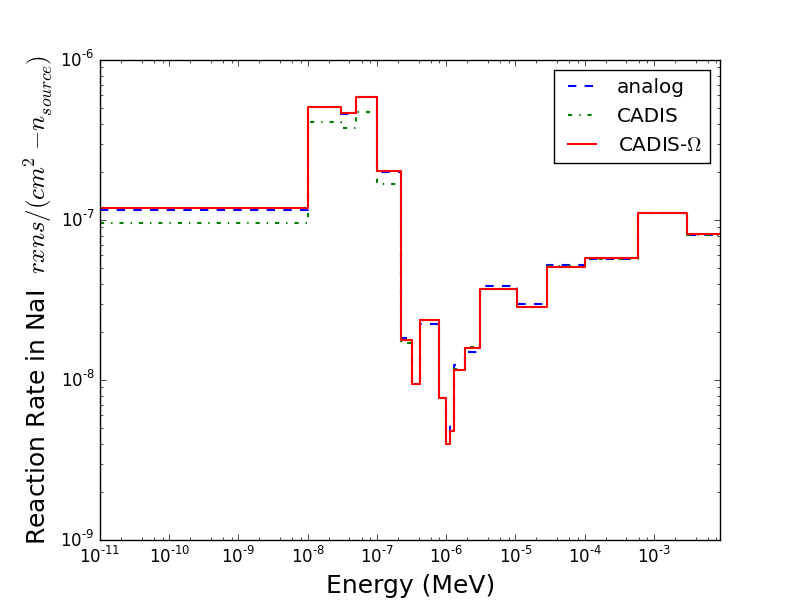
\includegraphics[height=1.3in,clip]{response.png}
		%\caption{Response for maze 2}
	\end{center}
  	\end{figure}
  	  \begin{figure}
  	\begin{center}
  		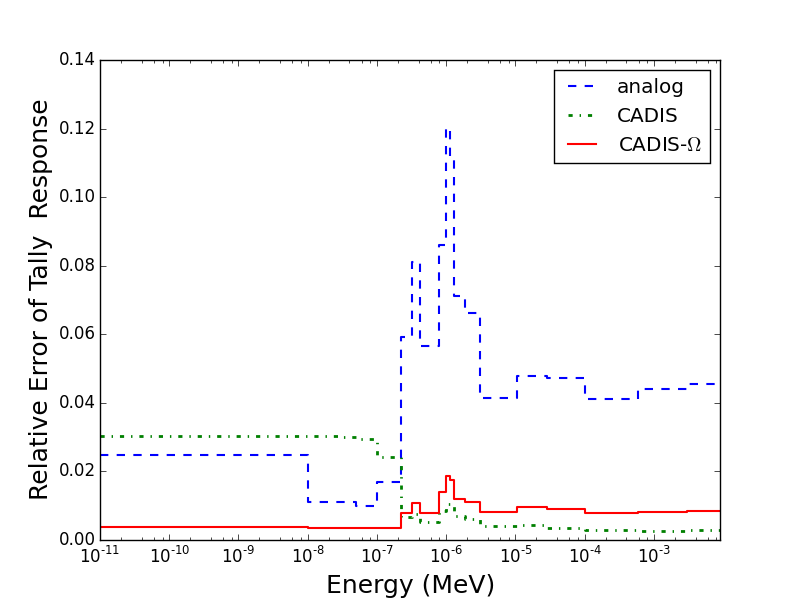
\includegraphics[height=1.3in,clip]{response_RE.png}
		%\caption{Relative errors for response function}
		% point out that while the FOM is better for analog, it has high RE in regions, so overall it performs poorer
	\end{center}
  	\end{figure}
  \end{column}
\end{columns}
	
\end{frame}

%% --------------------------------------------------------------
%% --------------------------------------------------------------
%\section{\scshape Continuing Work}
\begin{frame}[fragile]

  \frametitle{Characterization Tests}
   Quantify method's effectiveness and sensitivity for a variety of physics and concerns: \\
   \vspace*{.5 em}
    Streaming channels; \hspace*{2 em} Labyrinth variants;\\
    Spherical boat; \hspace*{4.25 em} Kobayashi benchmark
    \vspace{1 em}
    
    \begin{columns}
    \begin{column}{0.45\textwidth}
    \textbf{Deterministic}
    \begin{itemize}
    \item Energy groups 
    \item Quadrature order
    \item Quadrature type
    \item Spatial discretization
    \end{itemize}
    \end{column}
    
    \begin{column}{0.55\textwidth}
    \textbf{Monte Carlo}
    \begin{itemize}
    \item Tally spatial resolution (FW CADIS only)
    \item Tally energy resolution 
    \end{itemize}
    \end{column}
  \end{columns}

\end{frame}

%% --------------------------------------------------------------

\begin{frame}[fragile]

  \frametitle{Scaling Tests}
  
  Real system tests will show the ability of the method to improve MC for applications of interest
  \vspace*{1 em}
%  \begin{itemize}
%    \item Dry cask storage 
%    \item Active interrogation
%    \item Medical irradiation facility
%    \item PWR facility boundary
%  \end{itemize}

NEED PICTURE OF CASK  

\end{frame}

% --------------------------------------------------------------
% --------------------------------------------------------------


\section*{}
\begin{frame}[fragile]
  \frametitle{Questions?}
  \begin{center}
  \includegraphics[height=3in,clip]{../questions-comic}  
  \end{center}
  
\end{frame}

% --------------------------------------------------------------
\begin{frame}[allowframebreaks]{References}
	\bibliographystyle{unsrt}
	\bibliography{2015-03-mpact}
\end{frame}

\end{document}
